\documentclass[../main/main.tex]{subfiles}


\begin{document}

\section{April  9th, 2019}
\subsection*{Review}

\textbf{Steiner Forest problem} Given a graph $G=(v,E)$ with positive edge weights $c_e$ for each edge $e\in E$ and connectivity requirements \[
	r(u,v) = \begin{cases}
		1 \quad \text{if $u$, $v$ must be connected}\\ 0 \quad \text{otherwise}
	\end{cases}
.\] 





\begin{itemize}
	\item 
$S^{\star}$ : Collection of subsets $S\subseteq V$ such that for some $(u,v)$ for which some $r(u,v)=1$, for some $u\in S$ and $v\not\in  S$.
\item 
$\delta(S):$ Set of all edges crossing cut $(S,\overline{S}$.
\end{itemize}

\subsection{Primal Dual for Steiner Forest}
As an LP, this problem is: \\

\begin{centering}
	
\begin{tabular}{rl}
	minimize: &$\sum\limits_e c_e x_e$\\
	subject to: & $\sum\limits_{e:e\in \delta(S)} x_e\ge 1,\quad \forall  S\in S^{\star}$\\
				& $x_e\in \{0,1\} $
\end{tabular}\\
\end{centering}

Dual LP: \\

\begin{centering}
\begin{tabular}{rl}
	maximize& $\sum\limits_{S\in S^{\star}} y_s$\\
	subject to: & $\sum\limits_{S\in S^{\star}:e\in \delta(S)} y_s \le c_e,\quad \forall e\in E$\\
				& $y_s\ge 0$
\end{tabular}\\
	\end{centering}

In words, we are raising the dual of each set $S^{\star}$ while making sure that no edge leaving it is becoming over-tight.\\

The number of dual dual variables is equal to the number of cuts for which an edge must cross the cut, which could be exponential. However, many $y_s$ will remain 0, so it will still run in polynomial.\\

Consider the following:
\begin{figure}[h!]
	\centering
	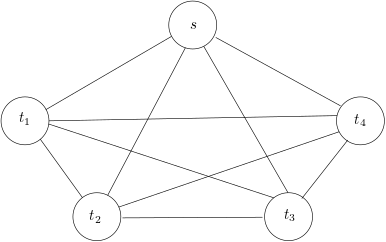
\includegraphics[width=0.8\textwidth]{4-9-dual-stf}
	\caption{Complete graph with all edges with weight 1. Note that all subsets are in $S^\star$ }
	\label{fig:4-9-stf}
\end{figure}
 \begin{itemize}
	\item Set $y_{\{t_1\} }=1$, picking all the edges leaving $t_1$. 
	\item Doing this, all sets in $S^{\star}$ will be satisfied, as they all have some $(t_1,v)$ crossing the cut.
	\item The solution has 5, but in general it might have $k$ (for  $K_k$). However, the lower bound is only 1, making the lower bound useless.
\end{itemize}
The break through idea is to raise the dual variable simultaneously. We can do this beaus any dual feasible solution is a valid lower bound, so we can grow the duals in any way. Note that for this example, we can raise all dual variables to 0.5, meaning our lower bound is $\frac{k+1}{2}$. (Note that we are only concerned with the $y_S$ for single term sets, with all others still 0).\\
\subsection{Approximation Algorithm for the Steiner Forest Problem}
\begin{remark}
	\textbf{NEW IDEA}: Raise duals in a synchronized manner. We are not trying to satisfy a singly unsatisfied primal constraint, but we are trying out many possibilities at the same time.
\end{remark}
This might seem ad hoc at first, but it turns out that it could be applied to many situations. Instead of raising one dual at a time, raise them all together.\\

\begin{remark}
	Terminology:
	\begin{itemize}
		\item We say that edge $e$ \vocab{feels} dual $y_s$ if $y_s>0$ and $e\in  \delta(S)$.
		\item We say that edge $e $ is \vocab{tight} if the total amount of dual it feels equals its cost, i.e. \[
				\sum\limits_{S\in S^\star:e\in \delta(S)} y_e=c_e
		.\] 
	\item We say that edge $s$ is \vocab{over-tight} if the total amount of dual it feels exceeds its cost.
	\item We say that a set $S$ has been \vocab{raised} if $y_S>0$
		
	\end{itemize}
\end{remark}
\begin{theorem}
	The dual is trying to maximize the sum of dual variables $y_S$ subject to the condition that no edge feels more dual than its cost - i.e. no edge is over-tight.
\end{theorem}

\begin{figure}[h!]
	\centering
	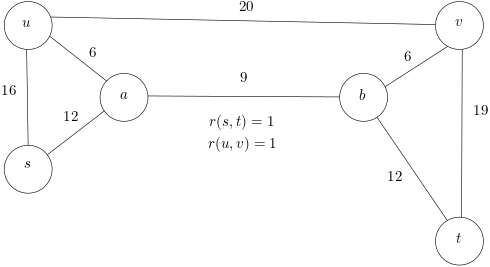
\includegraphics[width=0.8\textwidth]{4-9-stf-example}
	\caption{Optimal Solution: $(u,a),(s,a),(a,b),(b,t),(b,c)$}
\end{figure}
Let us consider how out algorithm will work with this example.
\begin{itemize}
	\item Let us consider the single vertex cuts of $\{u\} , \{s\} , \{v\} , \{t\} $. Note that $\{a\} , \{b\} \not\in S^\star$. We call $a,b$ \vocab{inactive components}
	\item We can raise all of these dual by 6, which will make $(u,a), (b,v)$ tight.
	\item If we follow the logic in the past, we might create a cycle, so for this example, we pick $(u,a)$. 
	\item This means that $\{s\} ,\{u,a\} ,\{v\} ,\{t\} $ are the new \vocab{active} components since they are in $S^{\star}$. 
	\item Now we raise the duals of the new active components, note that $\{u\} $ is inactive, but $\{u,a\} $ is active.
	\item We do this by going through all edges and finding the most serious constraint. Since $(v,b)$ is already tight, we raise them by 0 and pick $(v,b)$.
		 \begin{remark}
			For each iteration, we pick exactly one edge, and we are allowed to raise the duals by 0.
		\end{remark}
	\item We raise $\{s\} , \{u,a\} , \{v,b\} , \{t\} $ by 2, which makes $(s,u)$ tight, and so we pick it.
	\item Now we have three active components $\{u,a,s\} ,  \{v,b\} , \{t\} $, and we could raise them by 1, making $(b,t)$ tight.
		\begin{remark}
			Make sure you keep track if the edge is adjacent to 1 or 2 active components.
		\end{remark}
	\item Now we have two active components $\{u,a,s\} ,\{b,v,t\} $. We can raise them by 1 each, making $(u,v)$ tight.
	\item After this, we have 1 component which is inactive.
\begin{remark}
	After doing this, we need to check if every edge is needed, as some are redundant, e.g. $(u,a)$. (Special pruning step).
\end{remark}
\item The solution we return is $16+20+6+12=44$. 
\item The lower bound is $6\times 4+2\times 4+1\times 3+1\times 2=37$.
\end{itemize}
\begin{figure}[h!]
	\centering
	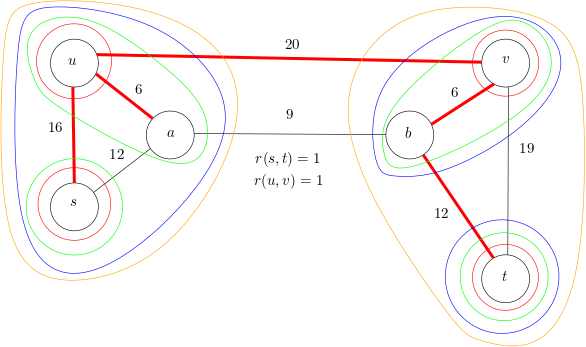
\includegraphics[width=0.8\textwidth]{4-9-stf-example-2}
	\caption{Example of the Algorithm}
\end{figure}
\begin{algo}

	\begin{itemize}
		\item Say the algorithm has picked some edges so far, which forms a forest $F$.
		\item We say that a set $S$ is \vocab{unsatisfied} if $S\in S^{\star}$ but there is no picked edge crossing the cut $(S,\overline{S})$. 
		\item Clearly if $F$ is not primal feasible, then there is a connected component in $F$ that is unsatisfied. We say that this component is \vocab{active}.
		\item In each iteration, we raise the dual of each active component until some edge goes tight. We pick one of the tight edges, and repeat.
		\item We stop when all connectivity requirements are satisfied, i.e. no sets are unsatisfied. 
		\item Finally do the pruning step by removing the redundant edges.
	\end{itemize}
\end{algo}

\end{document}


